\section{Results}
\label{sec:results}

\subsection{Primary scarce-label comparison}

\begin{table*}[t]
\centering
\footnotesize
\setlength{\tabcolsep}{4.5pt}
\caption{Primary held-out performance in the scarce-label regime (mean $\pm$ sample standard deviation over seeds 101--103). Test 1 uses temperature $R^2$; Tests 2--4 use water-saturation $R^2$. The last column is the difference between the two displayed means.}
\label{tab:primary_summary}
\begin{tabular}{@{}llrlll@{}}
\toprule
Test & Region & $N$ & Best PINN & Best classical & $\Delta R^2$ \\
\midrule
T1 & Interp. & 20 & H $0.997\pm0.002$ & GP $0.775\pm0.132$ & $+0.223$ \\
T1 & Interp. & 100 & H $1.000\pm0.000$ & GP $1.000\pm0.000$ & $+0.000$ \\
T1 & Forecast & 20 & H $0.955\pm0.016$ & SVR $0.395\pm0.363$ & $+0.560$ \\
T1 & Forecast & 100 & H $0.969\pm0.009$ & SVR $0.645\pm0.180$ & $+0.324$ \\
\addlinespace[1.5pt]
T2 & Interp. & 20 & HO $0.901\pm0.038$ & GP $0.564\pm0.105$ & $+0.337$ \\
T2 & Interp. & 100 & H $0.977\pm0.009$ & GP $0.859\pm0.045$ & $+0.118$ \\
T2 & Forecast & 20 & H $0.834\pm0.027$ & XGB $0.143\pm0.191$ & $+0.691$ \\
T2 & Forecast & 100 & HO $0.933\pm0.014$ & SVR $0.579\pm0.171$ & $+0.355$ \\
\addlinespace[1.5pt]
T3 & Interp. & 20 & HO $0.576\pm0.027$ & SVR $0.204\pm0.076$ & $+0.372$ \\
T3 & Interp. & 100 & H $0.840\pm0.014$ & GP $0.745\pm0.052$ & $+0.095$ \\
T3 & Forecast & 20 & HO $0.547\pm0.041$ & XGB $0.070\pm0.088$ & $+0.478$ \\
T3 & Forecast & 100 & H $0.780\pm0.052$ & XGB $0.491\pm0.072$ & $+0.289$ \\
\addlinespace[1.5pt]
T4 & Interp. & 20 & H $0.517\pm0.044$ & GP $0.058\pm0.129$ & $+0.459$ \\
T4 & Interp. & 100 & HO $0.720\pm0.017$ & XGB $0.474\pm0.108$ & $+0.246$ \\
T4 & Forecast & 20 & HO $0.632\pm0.019$ & XGB $-0.009\pm0.330$ & $+0.642$ \\
T4 & Forecast & 100 & HO $0.737\pm0.038$ & XGB $0.353\pm0.116$ & $+0.384$ \\
\bottomrule
\end{tabular}
\end{table*}


Table~\ref{tab:primary_summary} compares the strongest PINN and classical mean at \(N=20\) and \(N=100\); the complete five-method values are given in Tables~\ref{tab:primary_full_n20} and \ref{tab:primary_full_n100}. The ranking is consistent across benchmark difficulty. At \(N=20\), H-PINN attains an interpolation \(R^2\) of \(0.997\pm0.002\) for the analytical heat equation, whereas the strongest classical mean is \(0.775\pm0.132\) from GP. For water saturation, the best PINN scores are 0.901, 0.576, and 0.517 in Tests 2--4; the corresponding classical bests are 0.564, 0.204, and 0.058.

At \(N=100\), both H-PINN and GP have saturated the heat interpolation problem. The flow distinction remains: H/HO-PINN reaches 0.977, 0.840, and 0.720 on Tests 2--4, compared with classical bests of 0.859, 0.745, and 0.474. Forecasting is harder for the data-only models. For example, at \(N=20\), Test 2 H-PINN reaches \(0.834\pm0.027\), while XGB reaches \(0.143\pm0.191\); in Test 4 both PINN variants reach approximately 0.632, while all classical means are negative. The best PINN has the highest mean primary \(R^2\) in all 24 comparisons formed by four tests, two regions, and \(N\in\{20,50,100\}\).

\begin{table*}[t]
\centering
\scriptsize
\setlength{\tabcolsep}{2.6pt}
\caption{Target-resolved performance at $N=50$ (mean $\pm$ sample standard deviation over seeds 101--103). The classical entry is the family with the highest mean $R^2$ in that row; its MSE is shown in the corresponding column. Bold marks the best mean across all five methods.}
\label{tab:target_summary}
\begin{tabular}{@{}cllcccccc@{}}
\toprule
Target & Test & Region & H $R^2$ & HO $R^2$ & Classical $R^2$ & H MSE & HO MSE & Classical MSE \\
\midrule
$S_w$ & T2 & Interp. & $0.945\pm0.025$ & \textbf{$0.949\pm0.022$} & GP $0.793\pm0.052$ & $\num{1.35e-03}\pm\num{6.18e-04}$ & \textbf{$\num{1.24e-03}\pm\num{5.28e-04}$} & $\num{5.05e-03}\pm\num{1.27e-03}$ \\
$S_w$ & T2 & Forecast & $0.875\pm0.043$ & \textbf{$0.876\pm0.043$} & GP $0.569\pm0.228$ & $\num{4.33e-03}\pm\num{1.47e-03}$ & \textbf{$\num{4.30e-03}\pm\num{1.47e-03}$} & $\num{1.49e-02}\pm\num{7.87e-03}$ \\
$S_w$ & T3 & Interp. & $0.713\pm0.025$ & \textbf{$0.716\pm0.034$} & GP $0.562\pm0.178$ & $\num{4.29e-03}\pm\num{3.71e-04}$ & \textbf{$\num{4.25e-03}\pm\num{5.09e-04}$} & $\num{6.56e-03}\pm\num{2.67e-03}$ \\
$S_w$ & T3 & Forecast & \textbf{$0.657\pm0.033$} & $0.654\pm0.045$ & GP $0.470\pm0.147$ & \textbf{$\num{9.87e-03}\pm\num{9.63e-04}$} & $\num{9.96e-03}\pm\num{1.31e-03}$ & $\num{1.53e-02}\pm\num{4.24e-03}$ \\
$S_w$ & T4 & Interp. & \textbf{$0.633\pm0.031$} & $0.631\pm0.028$ & GP $0.342\pm0.055$ & \textbf{$\num{4.37e-03}\pm\num{3.67e-04}$} & $\num{4.39e-03}\pm\num{3.35e-04}$ & $\num{7.82e-03}\pm\num{6.58e-04}$ \\
$S_w$ & T4 & Forecast & \textbf{$0.680\pm0.040$} & $0.673\pm0.033$ & XGB $0.332\pm0.100$ & \textbf{$\num{8.48e-03}\pm\num{1.05e-03}$} & $\num{8.66e-03}\pm\num{8.81e-04}$ & $\num{1.77e-02}\pm\num{2.65e-03}$ \\
\midrule
$p$ & T2 & Interp. & $1.000\pm0.000$ & \textbf{$1.000\pm0.000$} & GP $0.998\pm0.001$ & $\num{4.11e-05}\pm\num{2.57e-05}$ & \textbf{$\num{3.71e-05}\pm\num{1.96e-05}$} & $\num{3.03e-04}\pm\num{1.14e-04}$ \\
$p$ & T2 & Forecast & $0.999\pm0.000$ & \textbf{$0.999\pm0.000$} & GP $0.995\pm0.002$ & $\num{1.57e-04}\pm\num{4.86e-05}$ & \textbf{$\num{1.39e-04}\pm\num{2.75e-05}$} & $\num{6.22e-04}\pm\num{2.83e-04}$ \\
$p$ & T3 & Interp. & \textbf{$0.991\pm0.002$} & \textbf{$0.991\pm0.003$} & GP $0.965\pm0.022$ & \textbf{$\num{8.06e-04}\pm\num{1.79e-04}$} & $\num{8.07e-04}\pm\num{2.24e-04}$ & $\num{3.11e-03}\pm\num{2.00e-03}$ \\
$p$ & T3 & Forecast & $0.979\pm0.005$ & \textbf{$0.979\pm0.004$} & GP $0.956\pm0.018$ & $\num{2.03e-03}\pm\num{5.17e-04}$ & \textbf{$\num{2.00e-03}\pm\num{4.26e-04}$} & $\num{4.19e-03}\pm\num{1.69e-03}$ \\
$p$ & T4 & Interp. & \textbf{$0.998\pm0.001$} & $0.998\pm0.001$ & GP $0.993\pm0.002$ & \textbf{$\num{2.68e-04}\pm\num{1.26e-04}$} & $\num{2.78e-04}\pm\num{1.19e-04}$ & $\num{1.01e-03}\pm\num{3.18e-04}$ \\
$p$ & T4 & Forecast & $0.996\pm0.001$ & \textbf{$0.996\pm0.001$} & GP $0.992\pm0.003$ & $\num{5.42e-04}\pm\num{1.91e-04}$ & \textbf{$\num{5.09e-04}\pm\num{1.89e-04}$} & $\num{1.20e-03}\pm\num{4.06e-04}$ \\
\bottomrule
\end{tabular}
\end{table*}


Table~\ref{tab:target_summary} resolves the flow comparison by target at the representative budget \(N=50\). A PINN has the best mean water-saturation \(R^2\) and MSE in all six test--region blocks. Pressure is easier for every method, but a PINN also leads all six pressure blocks. The separation is much larger for saturation: in Test 3 forecasting, H-PINN obtains water-saturation \(R^2=0.657\pm0.033\), compared with \(0.470\pm0.147\) for GP; their pressure scores are \(0.979\pm0.005\) and \(0.956\pm0.018\), respectively.

\subsection{Learning curves and label equivalence}

\begin{figure*}[t]
    \centering
    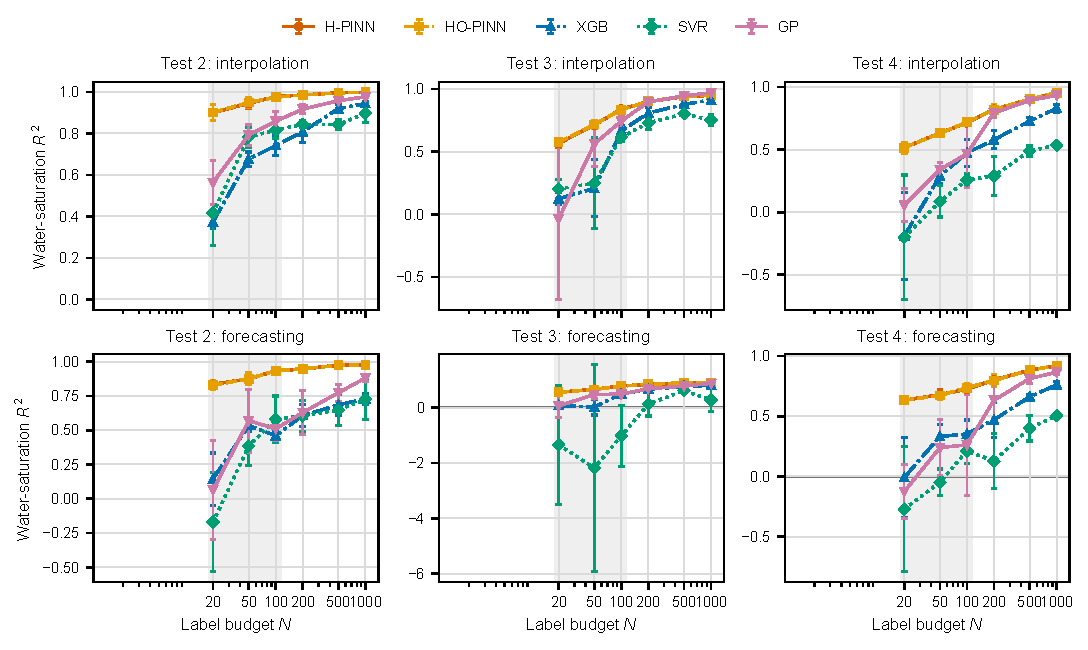
\includegraphics[width=\textwidth]{jcp_swat_r2_scaling.pdf}
    \caption{Water-saturation \(R^2\) versus labelled-state budget. Points and error bars are the mean and sample standard deviation over seeds 101--103. The grey band marks the prespecified small-data range \(N\le100\). Labels occupy the first 70\% of time; forecasting is evaluated on the final 30\%. Classical flow models are tuned by forward-time validation at every budget.}
    \label{fig:swat_scaling}
\end{figure*}

The flow learning curves in Fig.~\ref{fig:swat_scaling} show both the advantage and its boundary. Test 2 is PINN-dominated at every budget, although the interpolation margin decreases from 0.337 at \(N=20\) to 0.022 at \(N=1000\). Test 3 has the clearest crossover: the best PINN leads GP by 0.372, 0.154, and 0.095 at \(N=20,50,100\), is nearly tied at \(N=200\), and is slightly behind at \(N=500\) and \(N=1000\). Test 4 remains PINN-dominated because the same labels must cover space, time, and four physical parameters; its interpolation margin decreases from 0.459 at \(N=20\) to 0.021 at \(N=1000\).

\begin{table}[t]
\centering
\scriptsize
\setlength{\tabcolsep}{2.3pt}
\caption{Discrete label equivalence at $N=50$. $N^*_{\rm class}$ is the smallest tested budget at which any classical mean reaches the best PINN mean. Ratios are relative to 50 PINN labels.}
\label{tab:label_equivalence}
\begin{tabular}{@{}llclc@{}}
\toprule
Test & Region & PINN $R^2$ & $N^*_{\rm class}$ & Ratio \\
\midrule
T1 & Interp. & 0.999 & 100 (GP) & 2$\times$ \\
T1 & Forecast & 0.972 & $>1000$ & $>20\times$ \\
T2 & Interp. & 0.949 & 500 (GP) & 10$\times$ \\
T2 & Forecast & 0.876 & 1000 (GP) & 20$\times$ \\
T3 & Interp. & 0.716 & 100 (GP) & 2$\times$ \\
T3 & Forecast & 0.657 & 200 (GP) & 4$\times$ \\
T4 & Interp. & 0.633 & 200 (GP) & 4$\times$ \\
T4 & Forecast & 0.680 & 500 (GP) & 10$\times$ \\
\bottomrule
\end{tabular}
\end{table}


Table~\ref{tab:label_equivalence} expresses the same effect in label units. To match the best \(N=50\) PINN mean, a classical model requires 2--20 times more labels over seven of the eight test--region pairs. None reaches the heat-forecasting target by \(N=1000\). This is a discrete diagnostic over the tested budgets, not an interpolated sample-complexity estimate.

\begin{figure*}[t]
    \centering
    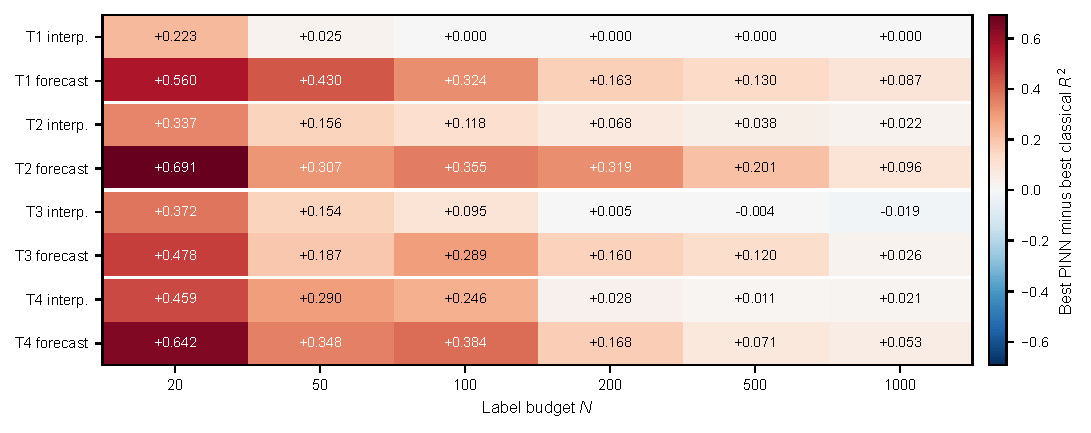
\includegraphics[width=\textwidth]{jcp_advantage_map.pdf}
    \caption{Difference between the best PINN and best classical mean \(R^2\) at every tested budget. Test 1 uses temperature; Tests 2--4 use water saturation. Positive values favour PINN.}
    \label{fig:advantage}
\end{figure*}

The advantage map in Fig.~\ref{fig:advantage} summarizes all 48 budget--test--region comparisons. The best PINN wins 43. All five classical wins are confined to interpolation: three negligible differences in the nearly solved heat problem and two Test 3 GP crossovers. A PINN has the highest mean in every temporal-forecasting comparison.

\begin{figure*}[t]
    \centering
    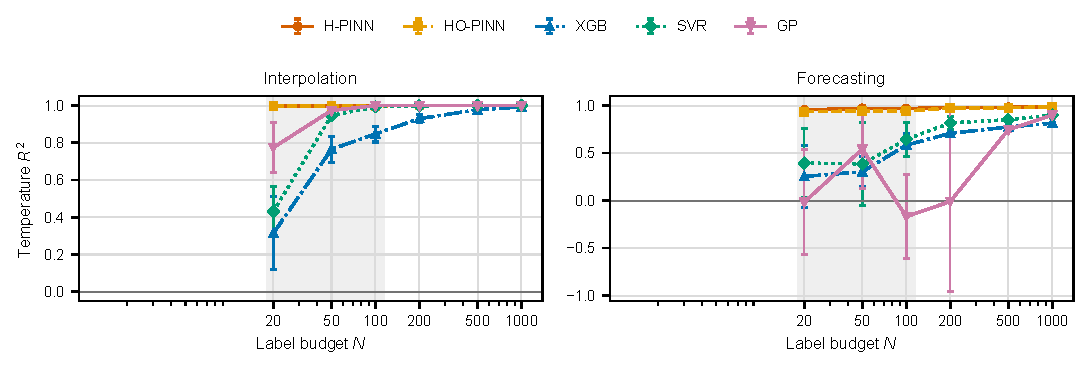
\includegraphics[width=\textwidth]{jcp_test1_r2_scaling.pdf}
    \caption{Temperature \(R^2\) for the analytical heat equation. The grey band marks \(N\le100\). GP becomes essentially exact for data-rich interpolation, whereas the PINN retains a clear equation-assisted forecasting advantage.}
    \label{fig:heat_scaling}
\end{figure*}

Figure~\ref{fig:heat_scaling} separates interpolation from forecasting on the smoothest benchmark. GP becomes essentially exact for interpolation from \(N=200\), but its future-time predictions remain unstable across sparse selections. H-PINN stays between 0.955 and 0.983 through \(N=20\)--500 because it enforces the heat operator beyond the latest labelled time.

\subsection{Qualitative reconstruction and physical admissibility}

\begin{figure}[H]
    \centering
    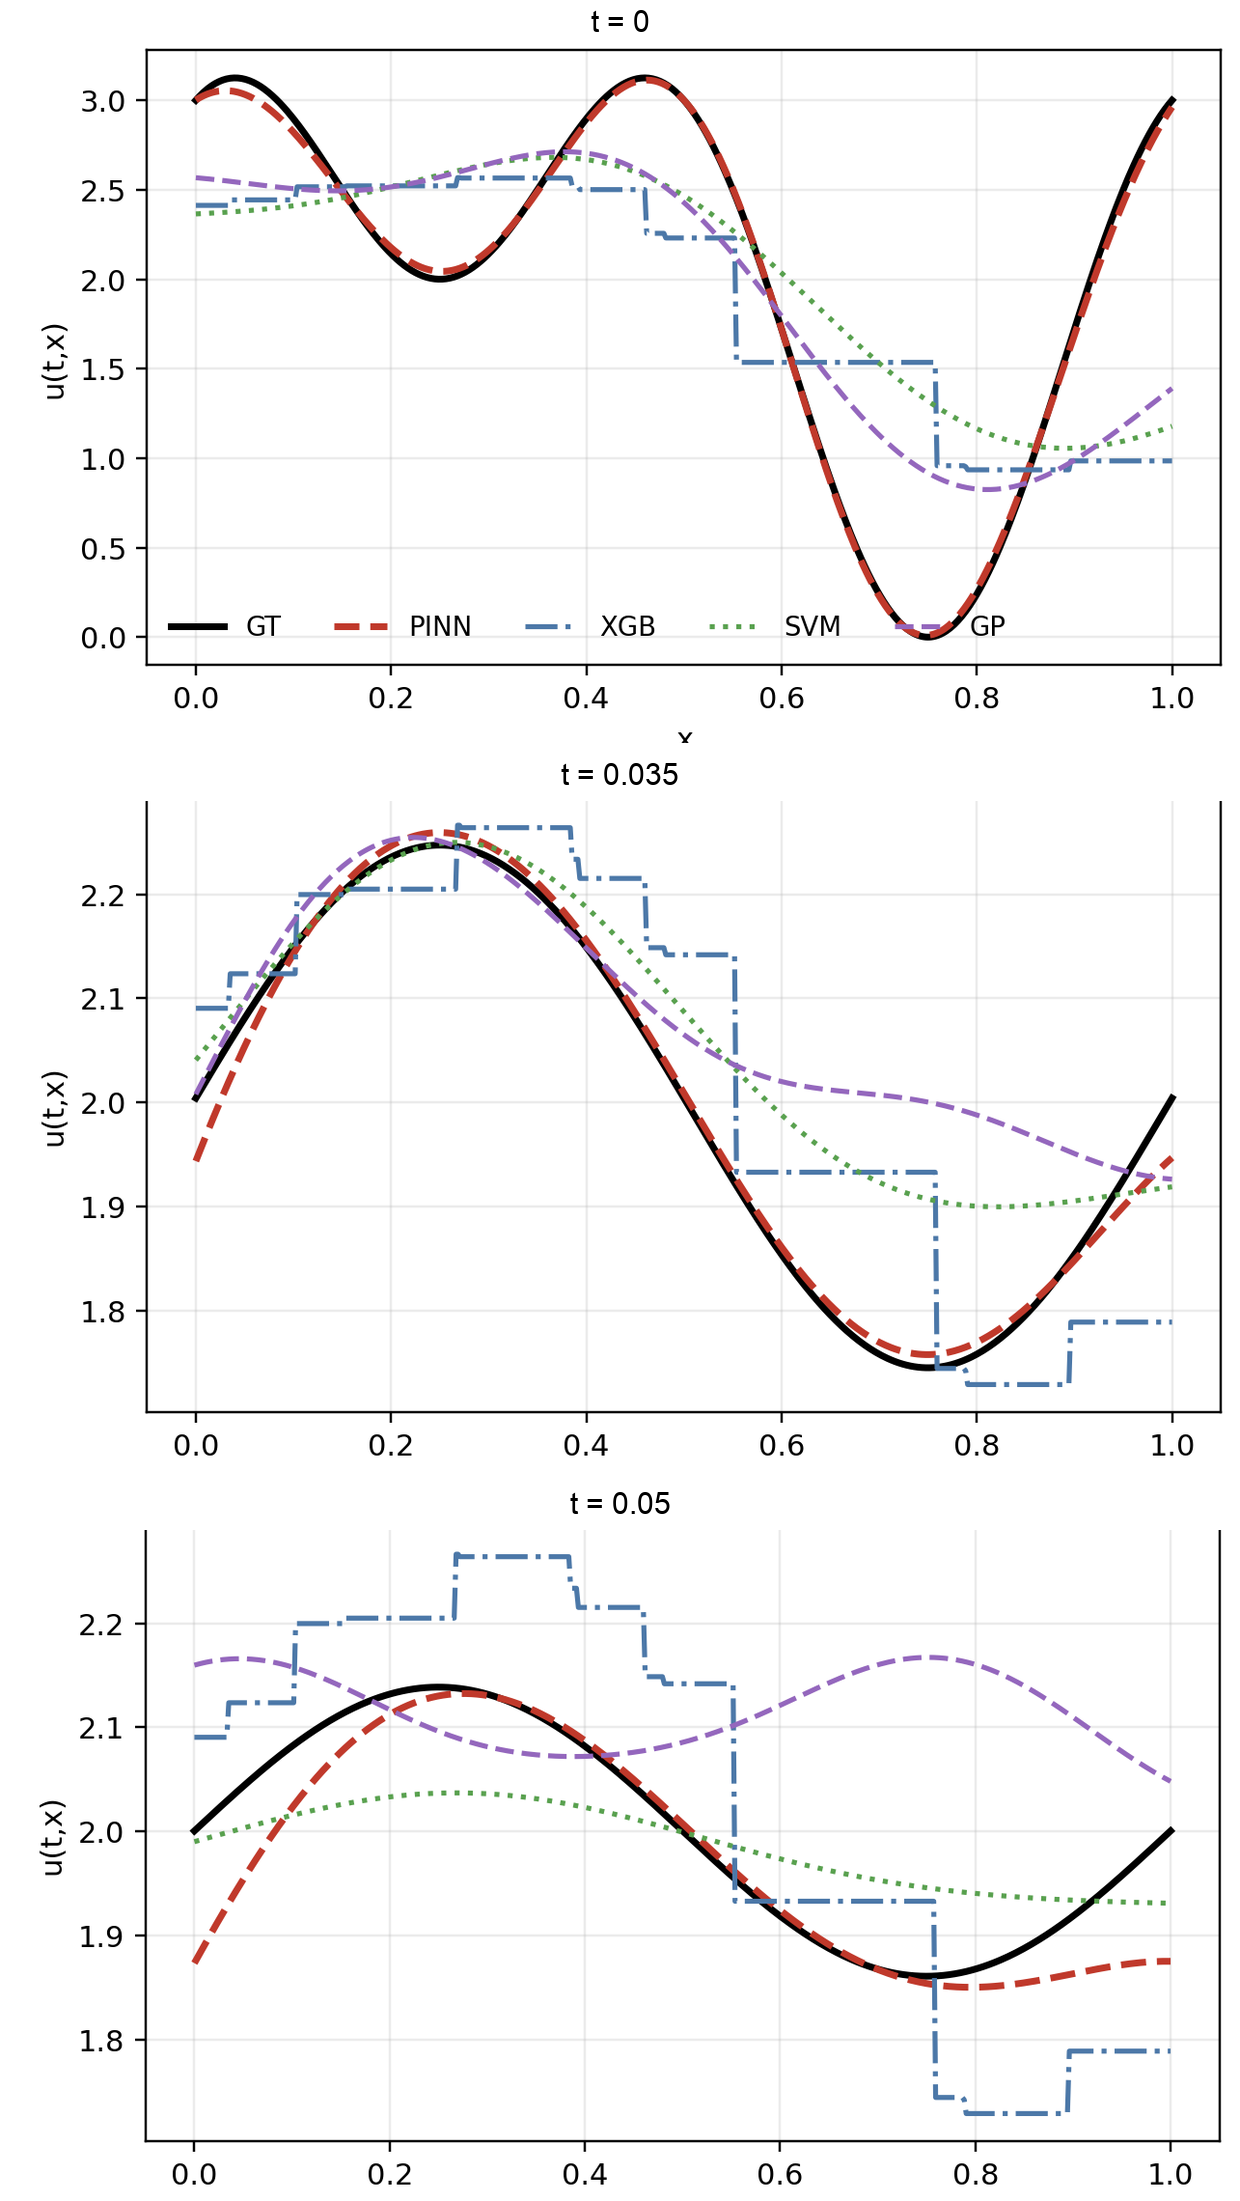
\includegraphics[width=0.90\columnwidth]{qualitative_test1_vertical.png}
    \caption{Test 1 profiles for seed 101 at \(N=20\): initial state (\(t=0\)), end of the labelled-time interval (\(t=0.035\)), and final forecast (\(t=0.05\)). H-PINN reconstructs the periodic modes and their dissipative evolution; XGB, SVR, and GP use the same labels but no equation residual.}
    \label{fig:qual_heat}
\end{figure}

The profiles in Fig.~\ref{fig:qual_heat} explain the heat scores. H-PINN preserves the correct modal decay from only 20 labels. XGB retains a piecewise-constant structure, while SVR and GP interpolate the observed interval smoothly but do not reproduce the final-time decay.

\begin{strip}
    \centering
    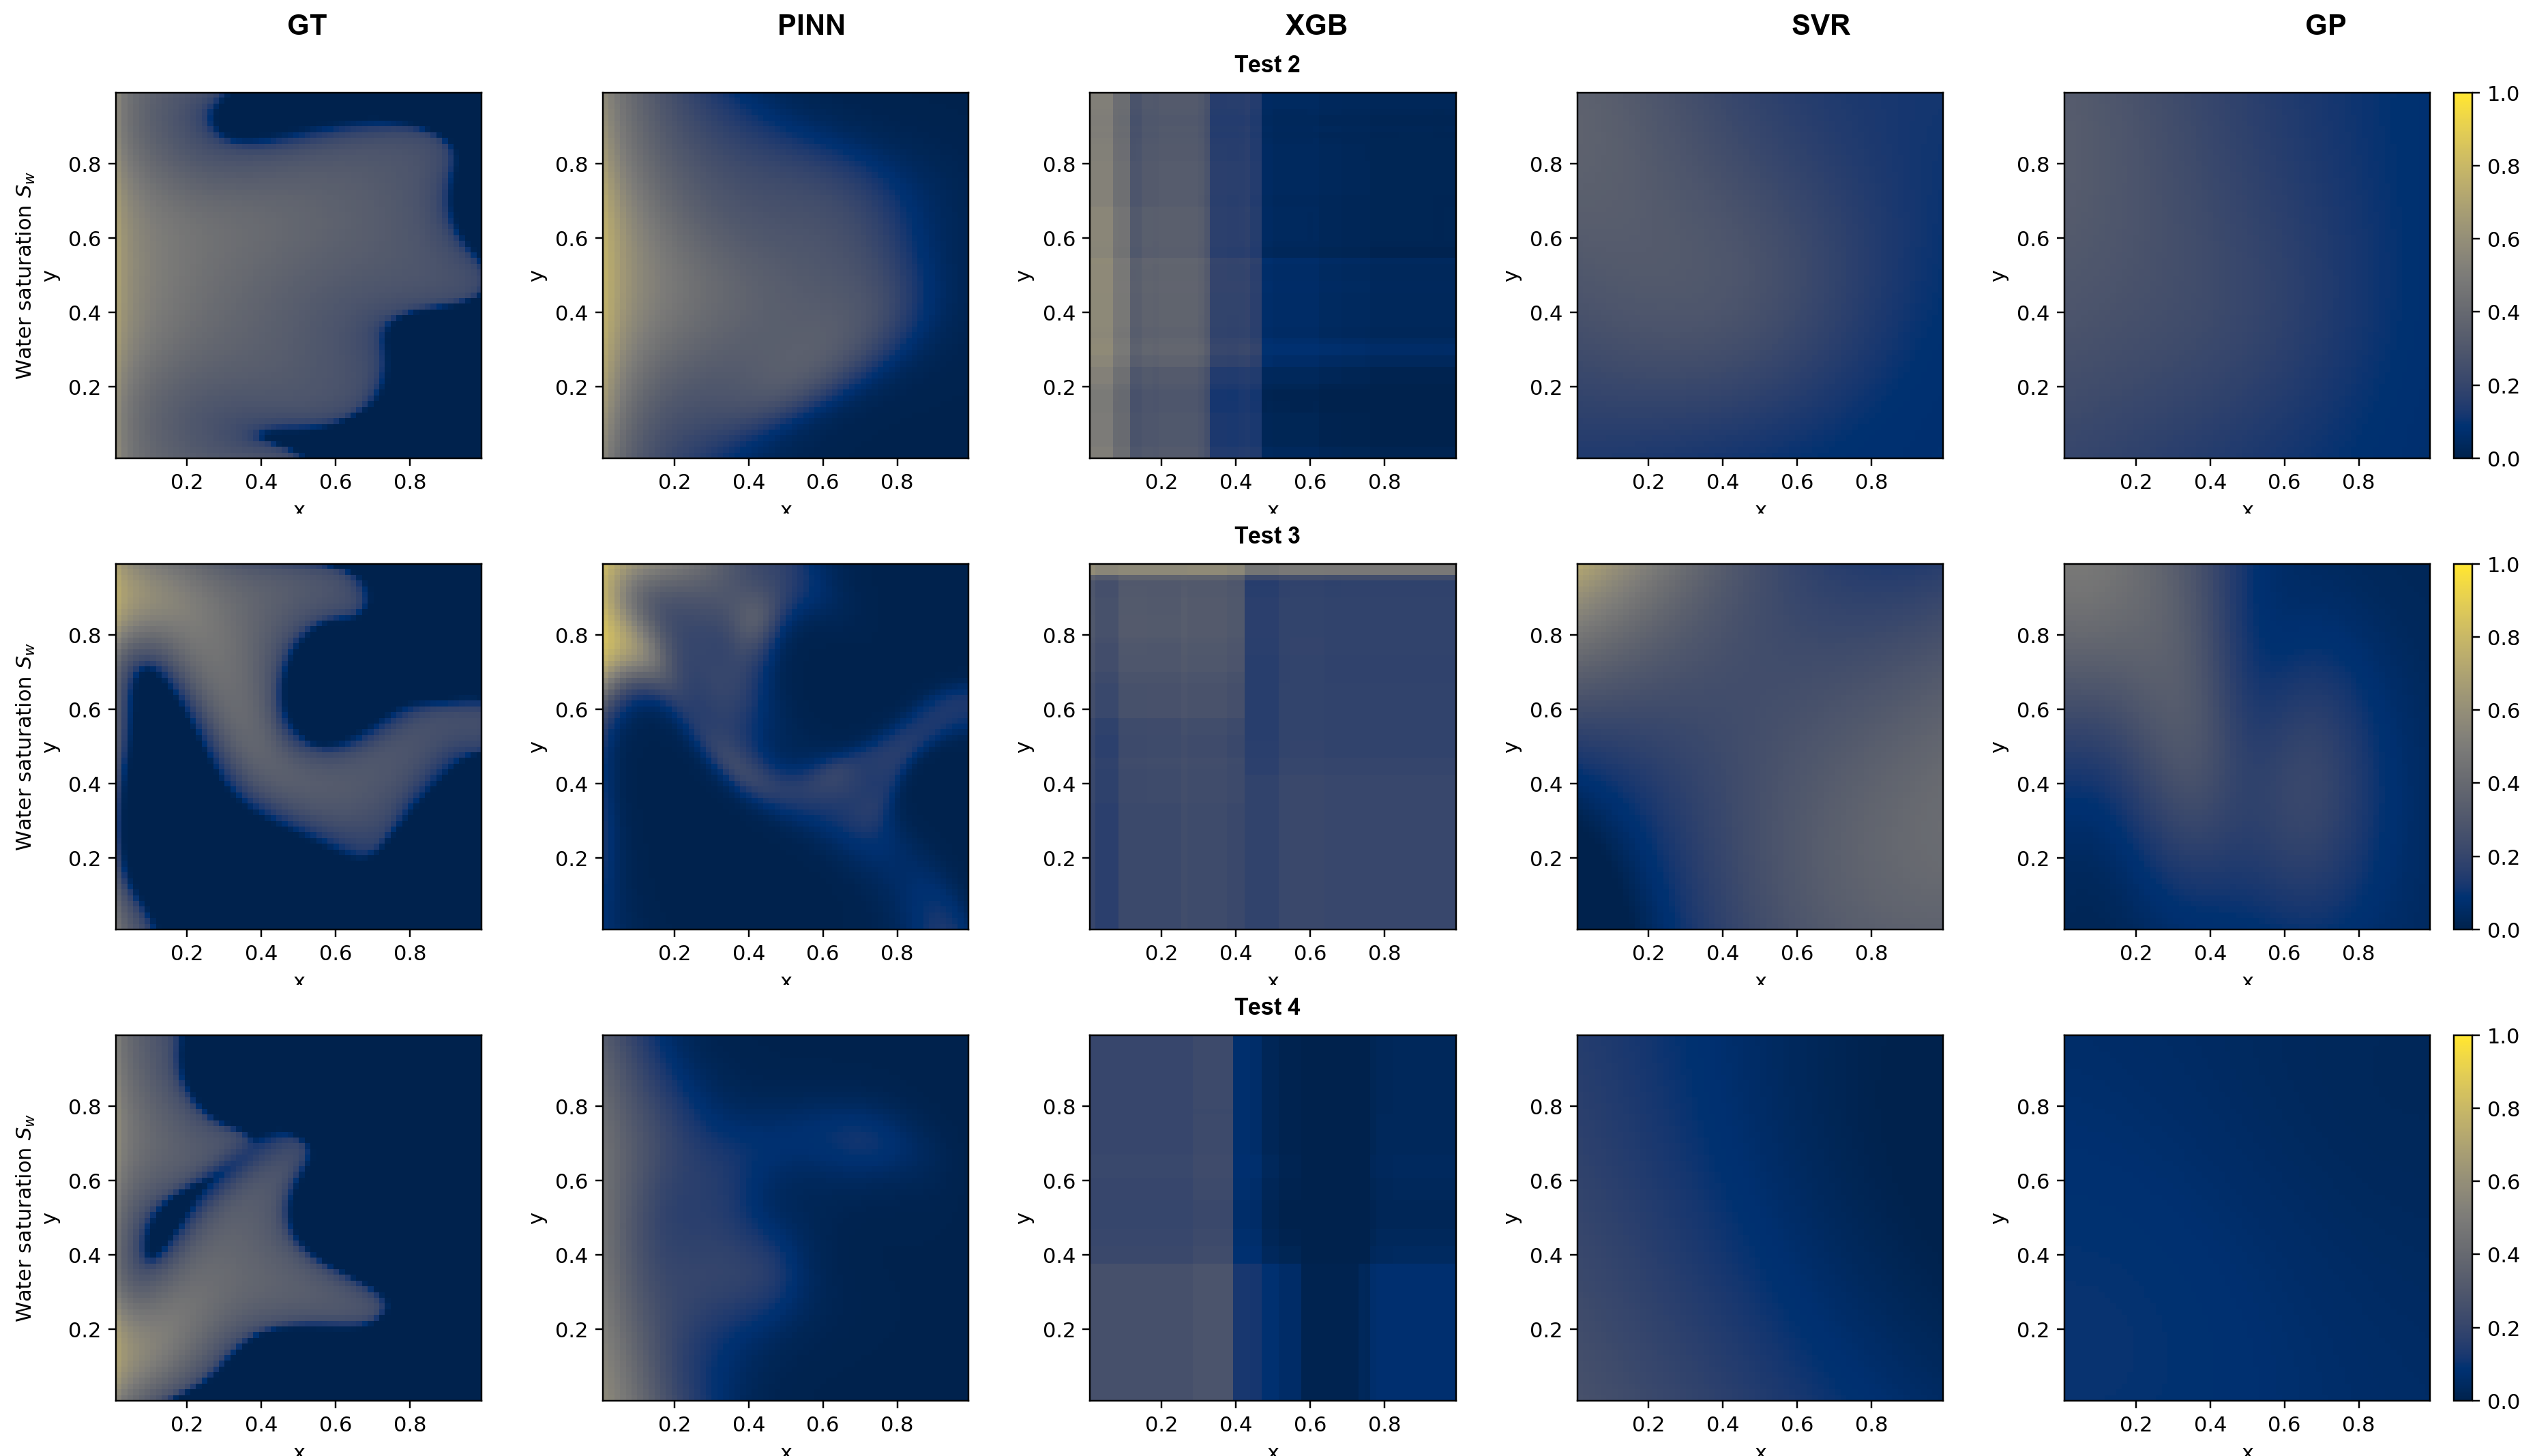
\includegraphics[width=0.96\textwidth]{qualitative_flow_saturation_composite.png}
    \captionsetup{hypcap=false}
    \captionof{figure}{Final forecasting-time water saturation for seed 101. Rows show Tests 2--4; columns compare the reference, H-PINN, XGB, SVR, and GP. Tests 2 and 3 use \(N=50\); Test 4 uses \(N=20\) and parameter realization 7. Colour limits are shared within every row.}
    \label{fig:qual_flow_saturation}
\end{strip}

The saturation fields in Fig.~\ref{fig:qual_flow_saturation} expose differences hidden by the easier pressure target (Appendix Fig.~\ref{fig:qual_flow_pressure}). H-PINN captures the displaced volume and broad front geometry in Test 2. In Test 3 it recovers the curved high-conductivity pathway; XGB is block-like, while SVR and GP smooth away much of the transported phase.

The Test 4 row is deliberately severe: 20 labelled states cannot explicitly cover 100 parameter combinations and a space--time domain. The classical saturation fields remain close to a low-amplitude average response. H-PINN does not reproduce every sharp feature, but predicts substantial displacement and its parameter-conditioned geometry, consistent with the positive forecasting \(R^2\).

The constrained output map gives zero saturation-bound violations in every flow run and closure MAE of approximately \(10^{-8}\). At \(N=50\), classical bounds-violation rates in the forecasting region range from 5.2\% to 18.6\% in Test 2, 3.7\% to 15.7\% in Test 3, and 1.3\% to 10.8\% in Test 4. These diagnostics (Table~\ref{tab:physical_diagnostics}) do not enter the accuracy ranking; they show that the PINN prediction is also physically admissible.

\subsection{Loss balancing and computational cost}

H-PINN and HO-PINN track one another closely throughout Fig.~\ref{fig:swat_scaling}. Neither uniformly dominates: HO-PINN is slightly better in several very sparse cases, whereas H-PINN is often equal or marginally stronger as \(N\) grows. The large scientific contrast is between either PINN and the classical models, not between the weighting variants. The simpler H-PINN alone has a higher mean than every classical baseline in all 24 comparisons at \(N\le100\).

The gain is not free. At \(N=50\), H-PINN fitting takes approximately 135--288 seconds and HO-PINN 216--448 seconds on the recorded hardware; complete classical tuning takes less than eight seconds and often less than one (Table~\ref{tab:runtime}). Thus, PINN is attractive when the cost of labels dominates
\begin{equation}
    C_{\mathrm{total}}(N)
    =N C_{\mathrm{label}}+C_{\mathrm{fit}}(N)+M C_{\mathrm{query}}(N),
\end{equation}
and the reduction in required \(N\) offsets the larger fitting cost. When labels are cheap and abundant, a tuned classical surrogate is operationally preferable.
